\documentclass[a4paper,oneside,12pt]{book}

% KODOVANI, CESTINA
\usepackage[utf8]{inputenc}
\usepackage[czech]{babel}
\usepackage{graphicx}
\usepackage{subcaption}

\DeclareGraphicsRule{*}{mps}{*}{}

% MATEMATIKA, CITACE, ...
\usepackage{amsthm}
\usepackage{amssymb}
\usepackage{enumerate}
\usepackage{hyperref}
\usepackage{cite}
\usepackage{amsmath}

% ODKAZY
\usepackage{hyperref}

% DEFINICNI BLOK
\theoremstyle{definition}
\newtheorem{df}{Definice}
\newtheorem*{zn}{Značení}
\newtheorem*{pr}{Příklad}

\theoremstyle{plain}
\newtheorem{vt}{Věta}
\newtheorem*{tv}{Tvrzení}
\newtheorem*{pz}{Pozorování}
\newtheorem{lm}{Lemma}
\newtheorem*{hp}{Hypotéza}

\theoremstyle{remark}
\newtheorem{po}{Poznámka}

%--------------------------------------------------

\begin{document}

% ---------------------------------- Obsah ----------------------------------- %
\tableofcontents

\setcounter{page}{1}

\pagebreak


% ----------------------------------- Úvod ----------------------------------- %
{
  \pagestyle{plain}
  
  \chapter*{Úvod}
\addcontentsline{toc}{chapter}{Úvod}

Matematické programování (optimalizace) se zabývá hledáním optimálních řešení matematických modelů. Modely, ve kterých se vyskytují pouze lineární funkce se zabývá lineární programování. Začátky lineárního programování jsou spojeny s druhou světovou válkou. George Dantzig, který měl na starosti vývoj logistických plánu na straně amerického letectva, v roce 1947 vymyslel Simplexovou metodu. S podobným konceptem přišel už dříve v roce 1939 Leonid Kantorovič, ale na jeho práci bohužel nikdo nenavázal. Další slavná jména, která stojí za zmínku v souvislosti s lineárním programováním jsou John von Neumann, Albert Tucker, Harold Kuhn a spousta dalších. Relativně nová oblast optimalizace se nazývá semidefinitní programování, kterou dobře charakterizuje název článku z roku 1981 s názvem \textit{Linear Programming with Matrix Variables} od Cravena a Monda. Pokud máme optimalizační problém, ve kterém řešení jsou vyjádřena pomocí diskrétních proměnných, pak hovoříme o problému kombinatorické optimalizace. K řešení těchto problémů se v posledních cca 30 letech rozšířilo semidefinitní programování, které se využívá např. u Shannonovy kapacity grafu, studia řezů, problému obchodního cestujícího a dalších. Pro další historické informace související s optimalizací doporučuji zdroj \cite{history}, ze kterého bylo čerpáno.
  
  \clearpage
}


% ---------------------------- ČÁST: OPTIMALIZACE----------------------------- %
\part{Optimalizace}

\chapter{Základní geometrické pojmy}

\section{Přímky a úsečky}

Mějme dva body $x_1, x_2 \in \mathbb{R}^n$ takové, že $x_1 \neq x_2$ a parametr $\theta \in \mathbb{R}$. Potom výraz
\begin{equation}
    y = \theta x_1 + (1 - \theta) x_2
    \label{line}
\end{equation}
popisuje \textbf{přímku} procházející body $x_1$ a $x_2$. Pro $\theta = 0$ dostáváme bod $x_2$ a pro $\theta = 1$ bod $x_1$. Omezíme-li $\theta$ na interval $\langle 0, 1 \rangle$, dostaneme \textbf{úsečku} s koncovými body $x_1$ a $x_2$. Výraz \ref{line} lze přepsat do tvaru
$$
    y = x_2 + \theta (x_1 - x_2),
$$
který můžeme interpretovat jako součet počátečního bodu $x_2$ a nějakého násobku směrového vektoru $x_1 - x_2$.

\section{Afinní prostory}

Říkáme, že $C \subseteq \mathbb{R}^n$ je \textbf{afinní prostor}, jestliže přímka procházející libovolnými dvěma různými body z $C$ leží v $C$. Tedy $C$ obsahuje lineární kombinace libovolných dvou bodů z $C$, jestliže součet koeficientů lineární kombinace je roven jedné. To lze zobecnit i pro více než dva body. Lineární kombinace $\theta_1 x_1 + \dots + \theta_k x_k$ bodů $x_1, \dots, x_k$ taková, že $\theta_1 + \dots + \theta_k = 1$, se nazývá \textbf{afinní kombinace} bodů $x_1, \dots, x_k$. Indukcí z definice afinního prostoru lze snadno ukázat, že pokud $C$ je afinní množina, $x_1, \dots, x_k \in C$ a $\theta_1 + \dots + \theta_k = 1$, potom bod $\theta_1 x_1 + \dots + \theta_k x_k \in C$.

\noindent Nechť $C$ je afinní prostor a $x_0 \in C$, potom množina
$$
    V = C - x_0 = \left\{ x - x_0 \mid c \in C \right\}
$$
je \textbf{lineární vektorový prostor}, tj. množina, která je uzavřená na sčítání a násobení skalárem.

\noindent Afinní prostor $C$ lze vyjádřit jako
$$
    C = V + x_0 = \left\{ v + x_0 \mid v \in V \right\},
$$
kde $V$ je vektorový prostor a $x_0$ je počátek. Poznamenejme, že vektorový prostor $V$ asociovaný s afinním prostorem $C$ nezávisí na volbě počátku $x_0$.

\noindent \textbf{Dimenze} afinního prostoru $C = V + x_0$ je definována jako dimenze vektorového prostoru $V = C - x_0$, kde $x_0$ je libovolný prvek z $C$. Množina všech afinních kombinací bodů množiny $C \subseteq \mathbb{R}^n$ se nazývá \textbf{afinní obal} množiny $C$. Afinní obal množiny $C$ budeme značit
$$
    \textbf{aff } C = \left\{ \theta_1 x_1 + \dots + \theta_k x_k \mid x_1, \dots, x_k \in C, \theta_1 + \dots + \theta_k = 1 \right\}.
$$
Afinní obal je nejmenší afinní prostor, který obsahuje množinu $C$. Tedy, jestliže $S$ je afinní prostor takový, že $C \subseteq S$, potom $\textbf{aff }C \subseteq S$.


\section{Konvexní množiny}

Říkáme, že množina $C$ je \textbf{konvexní}, jestliže úsečka mezi libovolnými dvěma body z $C$ leží také celá v $C$. Jinak řečeno, jestliže pro libovolné dva body $x_1, x_2 \in C$ a libovolné $\theta \in \langle 0, 1 \rangle$ platí, že $\theta x_1 + (1 - \theta) x_2 \in C$. Poznamenejme, že každý afinní prostor je zároveň konvexní množinou. Podobně jako afinní kombinaci definujeme \textbf{konvexní kombinaci} bodů $x_1, \dots, x_k$ jako $\theta_1 x_1 + \dots + \theta_k x_k$, kde $\theta_1 + \dots + \theta_k = 1, \theta_i \geq 0$ pro $i = 1, \dots, k$. \textbf{Konvexní obal} množiny $C$ je množina všech konvexních kombinací bodů z množiny $C$, značíme
$$
    \textbf{conv }C = \left\{ \theta_1 x_1 + \dots + \theta_k x_k \mid x_i \in C, \theta_i \geq 0, i = 1, \dots, k, \theta_1 + \dots + \theta_k = 1 \right\}.
$$
Analogicky, konvexní obal množiny $C$ je nejmenší konvexní množina, která obsahuje množinu $C$. Pro představu viz obrázek~\ref{fig:convex_hull}.

\begin{figure}[h!]
    \centering
    \begin{subfigure}[b]{0.3\textwidth}
        \centering
        \includegraphics[width=\textwidth]{img/points_for_convex_hull.png}
        \caption{Množina bodů $C$}
        \label{fig:convex_hull:a}
    \end{subfigure}

    \hfill

    \begin{subfigure}[b]{0.3\textwidth}
        \centering
        \includegraphics[width=\textwidth]{img/convex_hull.png}
        \caption{$\textbf{conv }C$}
        \label{fig:convex_hull:b}
    \end{subfigure}
     
    \caption{Konvexní obal množiny}
    \label{fig:convex_hull}
\end{figure}


\section{Kužely}

Množina $C$ se nazývá \textbf{kužel}, jestliže pro každé $x \in C$ a $\theta \geq 0$ platí, že $\theta x \in C$. Je-li $C$ navíc konvexní, pak se $C$ nazývá \textbf{konvexní kužel}. Tedy $C$ je konvexní kužel, jestliže pro libovolné $x_1, x_2 \in C$ a $\theta_1, \theta_2 \geq 0$ platí, že $\theta_1 x_1 + \theta_2 x_2 \in C$. Říkáme, že bod ve tvaru $\theta_1 x_1 + \dots + \theta_k x_k$, kde $\theta_1, \dots, \theta_k \geq 0$ je \textbf{kuželovou kombinací} bodů $x_1, \dots, x_k$. Dále, pokud $x_i$ leží v konvexním kuželu množiny $C$, potom libovolná kuželová kombinace bodu $x_i$ leží rovněž v konvexním kuželu množiny $C$. Platí, že množina $C$ je konvexní kužel právě tehdy, když $C$ obsahuje všechny kuželové kombinace svých bodů. \textbf{Kuželový obal} množiny $C$ je množina, která obsahuje všechny kuželové kombinace množiny $C$, tj.
$$
    \textbf{cone }C = \left\{ \theta_1 x_1 + \dots + \theta_k x_k \mid x_i \in C, \theta_i \geq 0, i = 1, \dots, k \right\}.
$$
Kuželový obal množiny $C$ je zároveň nejmenší konvexní kužel, který obsahuje množinu $C$. Pro představu viz obrázek~\ref{fig:cone_hull}.

\begin{figure}[h!]
    \centering
    \begin{subfigure}[b]{0.3\textwidth}
        \centering
        \includegraphics[width=\textwidth]{img/points_for_cone_hull.png}
        \caption{Množina bodů $C$}
        \label{fig:cone_hull:a}
    \end{subfigure}

    \hfill

    \begin{subfigure}[b]{0.3\textwidth}
        \centering
        \includegraphics[width=\textwidth]{img/cone_hull.png}
        \caption{$\textbf{cone }C$}
        \label{fig:cone_hull:b}
    \end{subfigure}
     
    \caption{Kuželový obal množiny}
    \label{fig:cone_hull}
\end{figure}

\section{Nadroviny a poloprostory}

\textbf{Nadrovina} je množina ve tvaru
$$
    \left\{ x \mid a^T x = b \right\},
$$
kde $a \in \mathbb{R}^n$, $a \neq 0$ a $b \in \mathbb{R}$. Analyticky na nadrovinu nahlížíme jako na množinu všech řešení lineární rovnice. Geometricky zase jako na množinu všech bodů takových, že mají konstantní skalární součin s normálovým vektorem $a$. Konstanta $b$ značí posunutí nadroviny od počátku. Nadrovinu také můžeme vyjádřit jako
$$
    \left\{ x \mid a^T (x - x_0) = 0 \right\} = x_0 + \left\{ v \mid a^T v = 0 \right\},
$$
kde $x_0$ je libovolný bod této nadroviny a $\left\{ v \mid a^T v = 0 \right\}$ je množina všech vektorů, které jsou kolmé k normálovému vektoru $a$. Nadrovina je tedy množina, která obsahuje bod $x_0$ a libovolný bod ve tvaru $x_0 + v$, kde $v$ je vektor, který je kolmý k normálovému vektoru $a$. Pro ilustraci v $\mathbb{R}^2$ viz obrázek~\ref{fig:hyperplane}.

Nadrovina dělí $\mathbb{R}^n$ na dva poloprostory. Množina 
$$
    \left\{ x \mid a^T x \leq b \right\}, \text{ resp. } \left\{ x \mid a^T x < b \right\},
$$
kde $a \neq 0$ se nazývá (uzavřený) \textbf{poloprostor}, resp. \textbf{otevřený poloprostor}. Je to tedy množina všech řešení lineární nerovnice. Podobně jako nadrovinu, můžeme poloprostor vyjádřit ve tvaru
$$
    \left\{ x \mid a^T (x - x_0) \leq 0 \right\}, \text{ resp. } \left\{ x \mid a^T (x - x_0) < 0 \right\},
$$
kde $a \neq 0$ a $x_0$ je libovolný bod z nadroviny $\left\{ x \mid a^T x = b \right\}$. Poloprostor tedy obsahuje bod $x_0$ a libovolný bod $x_0 + v$, kde $v$ je vektor, který s vnějším normálovým vektorem svírá tupý nebo pravý úhel. Tato interpretace je v $\mathbb{R}^2$ ilustrována na obrázku~\ref{fig:halfspace}. Ještě poznamenejme, že poloprostory jsou konvexní množiny, ale samozřejmě nejsou afinní.

\begin{figure}[h!]
    \centering
    \begin{subfigure}[b]{0.3\textwidth}
        \centering
        \includegraphics[width=\textwidth]{img/hyperplane.jpg}   
        \caption{Nadrovina}
        \label{fig:hyperplane}
    \end{subfigure}

    \hfill

    \begin{subfigure}[b]{0.3\textwidth}
        \centering
        \includegraphics[width=\textwidth]{img/halfspace.jpg}   
        \caption{Poloprostor}
        \label{fig:halfspace}
    \end{subfigure}

    \caption{Nadrovina a poloprostor v $\mathbb{R}^2$.}
    \label{fig:hyperplane_halfspace}
\end{figure}

\section{Polyedry a polytopy}

Polytopy jsou zobecněním konvexních mnohoúhelníků v rovině do více dimenzí. Polytop v $\mathbb{R}^3$ je konvexní množina, která je ohraničena konečně mnoha konvexními mnohoúhelníky (příkladem polytopů v $\mathbb{R}^3$ jsou např. Platónská tělesa). Na takovou množinu je možné nahlížet dvěma způsoby. \textbf{H-polyedr} je průnik konečně mnoha uzavřených poloprostorů v $\mathbb{R}^n$. \textbf{H-polytop} je omezený H-polyedr. \textbf{V-polytop} je konvexní obal konečně mnoha bodů v $\mathbb{R}^n$. Následující věta říká, že H-polytop a V-polytop jsou matematicky ekvivalentní množiny.

\begin{vt2}\textbf{[REF]}
    Každý V-polytop je H-polytop. Každý H-polytop je V-polytop.
\end{vt2}

Poznamenejme, že V-polytop a H-polytop jsou sice ekvivalentní množiny, ale z algoritmického hlediska je velký rozdíl, zda pracujeme s bodovou množinou, nebo s uzavřenými poloprostory. Pro ilustraci: mějme lineární funkci, kterou chceme minimalizovat na daném polytopu. Pro V-polytop se jedná o triviální problém, protože stačí pro každý bod z množiny $V$ určit hodnotu dané funkce a vybrat minimum. Na druhou stranu pro H-polytop se jedná o netriviální problém, kterým se zabývá lineární programování. Dále budeme mluvit jen o \textbf{polyedrech} a \textbf{polytopech}.

Důležitý fakt, že každý polyedr je konečně generovaný, říká Minkowského-Weylova věta.
\begin{vt2}[Minkowski-Weyl]
    $P \subseteq \mathbb{R}^n$. Potom $P = \textbf{conv}(u_1, \dots, u_r) + \textbf{cone}(v_1, \dots, v_s)$, kde $u_i, v_i$ jsou extremální vrcholy $P$ právě tehdy, když $P = \left\{ x \in \mathbb{R}^n \mid Ax \leq b \right\}, A \in \mathbb{R}^{m \times n}, b \in \mathbb{R}^m$.
\end{vt2}


\chapter{Konvexní optimalizace}

Kapitola je zpracována z \cite{convex-optimization}.

\section{Obecná podmíněná úloha}

\begin{equation}\label{eq:constrained_problem}
    \begin{split}
        &\inf\ f(x) \\
        &g_i(x) \leq 0, i = 1, \dots, m \\
        &h_i(x) = 0, i = 1, \dots, p
    \end{split}
\end{equation}

Hledáme $x \in \mathbb{R}^n$, které minimalizuje $f(x)$, vzhledem k omezením $g_i(x)$ a $h_i(x)$. Proměnné $x$ říkáme \textbf{optimalizační proměnná}, funkci $f(x)$ říkáme \textbf{cenová} nebo \textbf{účelová funkce}. Výrazy $g_i(x) \leq 0$ jsou \textbf{omezení typu nerovnosti} a $h_i(x) = 0$ jsou \textbf{omezení typu rovnosti}. Říkáme, že problém~\ref{eq:constrained_problem} je \textbf{úloha nepodmíněné optimalizace}, jestliže $m = p = 0$. Jinak se jedná o \textbf{úlohu podmíněné optimalizace}.

\textbf{Definiční obor} $\mathcal{D}$ úlohy~\ref{eq:constrained_problem} je
$$
    \mathcal{D} = \bigcap_{i=1}^m \textbf{dom}\ g_i \cap \bigcap_{i=1}^p \textbf{dom}\ h_i.
$$
Říkáme, že bod $x \in \mathcal{D}$ je \textbf{přípustný}, jestliže splňuje všechna omezení $g_i(x) \leq 0$ a $h_i(x) = 0$. Úloha~\ref{eq:constrained_problem} je \textbf{přípustná}, jestliže existuje alespoň jeden bod $x \in \mathcal{D}$, který je přípustný. Množina všech přípustných bodů $x \in \mathcal{D}$ se nazývá \textbf{přípustná množina}.

\textbf{Optimální hodnota} $f^*$ úlohy~\ref{eq:constrained_problem} je definována jako
$$
    f^* = \inf \left\{ f(x) \mid g_i(x) \leq 0, i = 1, \dots, m, h_i(x) = 0, i = 1, \dots, p \right\}.
$$

\section{Konvexní podmíněná úloha}

\begin{equation}\label{eq:convex_problem}
    \begin{split}
        &\inf\ f(x) \\
        &g_i(x) \leq 0, i = 1, \dots, m \\
        &a_i^Tx = b_i, i = 1, \dots, p
    \end{split}
\end{equation}

Oproti obecné úloze~\ref{eq:constrained_problem} jsou funkce $f(x), g_i(x)$ konvexní a funkce $h_i(x) = a_i^Tx - b_i$ jsou afinní. Přípustná množina takové úlohy je konvexní množinou.

\section{Lagrangeova dualita}

Mějme úlohu~\ref{eq:constrained_problem} s $\mathcal{D} \neq \emptyset$. Zobrazení $L:\ \mathbb{R}^n \times \mathbb{R}^m \times \mathbb{R}^p \rightarrow \mathbb{R}$ takové, že
\begin{equation}
    L(x, \lambda, \mu) = f(x) + \sum_{i=1}^m \lambda_i g_i(x) + \sum_{i=1}^p \mu_i h_i(x)
\end{equation}
se nazývá \textbf{Lagrangeova funkce}. Definiční obor $\textbf{dom}\ L = \mathcal{D} \times \mathbb{R}^m \times \mathbb{R}^p$. Vektory $\lambda = (\lambda_1, \dots, \lambda_m)$ a $\mu = (\mu_1, \dots, \mu_p)$ nazýváme \textbf{duální proměnné} a prvkům těchto vektorů říkáme \textbf{Lagrangeovy multiplikátory}. Dále definujeme \textbf{duální funkci}
$$
    d:\ \mathbb{R}^m \times \mathbb{R}^p \rightarrow \mathbb{R}
$$
jako infimum Lagrangeovy funkce $L$ přes všechna $x \in \mathcal{D}$. Tedy
\begin{equation}
    d(\lambda, \mu) = \inf_{x \in \mathcal{D}} L(x, \lambda, \mu) = \inf_{x \in \mathcal{D}} \left( f(x) + \sum_{i=1}^m \lambda_i g_i(x) + \sum_{i=1}^p \mu_i h_i(x) \right).
\end{equation}

Poznamenejme, že duální funkce je konkávní bez ohledu na to, zda je úloha konvexní a je-li $L$ zdola neomezená v proměnné $x$, potom duální funkce nabývá hodnoty $-\infty$.

\subsection*{Dolní odhad na $f^*$}\label{s:lower_bound}

Nechť $\tilde{x}$ je přípustný bod. Pro $\lambda \geq 0$ je
$$
    \sum_{i=1}^m \lambda_i g_i(\tilde{x}) + \sum_{i=1}^p \mu_i h_i(\tilde{x}) \leq 0.
$$
Potom pro Lagrangeovu funkci můžeme psát
$$
    L(\tilde{x}, \lambda, \mu) = f(\tilde{x}) + \sum_{i=1}^m \lambda_i g_i(\tilde{x}) + \sum_{i=1}^p \mu_i h_i(\tilde{x}) \leq f(\tilde{x}).
$$
A tedy pro duální funkci platí
$$
    d(\lambda, \mu) = \inf_{x \in \mathcal{D}} L(x, \lambda, \mu) \leq L(\tilde{x}, \lambda, \mu) \leq f(\tilde{x}).
$$

\subsection*{Duální úloha}

V části~\ref{s:lower_bound} jsme si ukázali, že duální funkce dává dolní odhad na optimální hodnotu $x^*$ úlohy~\ref{eq:constrained_problem}. Stále jsme si ale neřekli, jaký je nejlepší dolní odhad, který pomocí duální funkce jsme schopni dostat. To nás dostává k následující optimalizační úloze.
\begin{equation}\label{eq:dual_problem}
    \begin{split}
        &\sup d(\lambda, \mu) \\
        &\lambda \geq 0
    \end{split}
\end{equation}

Úloze~\ref{eq:dual_problem} se říká \textbf{Lagrangeova duální úloha} příslušná k úloze~\ref{eq:constrained_problem}, kterou nazýváme \textbf{primární úlohou}.

\subsection*{Slabá dualita}

Optimální řešení Lagrangeovy duální úlohy označíme $d^*$, které je už z definice nejlepší dolní odhad na optimální řešení primární úlohy $f^*$. Tato nerovnost platí i pokud primární úloha není konvexní. Této nerovnosti říkáme \textbf{slabá dualita}. Rozdíl optimálních řešení $f^* - d^*$ označujeme jako \textbf{optimální dualitní rozdíl} primární úlohy. Poznamenejme, že optimální dualitní rozdíl je vždy nezáporný.


\subsection*{Silná dualita a Slaterova podmínka}

Pokud je optimální dualitní rozdíl $f^* - d^* = 0$, pak říkáme, že platí silná dualita. Silná dualita obecně neplatí, ale pro primární úlohu, která splňuje nějaké další podmínky to možné je. Těmto podmínkám se říká \textbf{podmínky kvalifikace omezení}. Jednou takovou je \textbf{Slaterova podmínka}
$$
    \exists x \in \textbf{relint}\ \mathcal{D}:\ g_i(x) < 0, i = 1, \dots, m, Ax = b.
$$

Bodu $x \in \mathcal{D}$, který splňuje Slaterovu podmínku, říkáme, že je \textbf{striktně přípustný}, protože omezení typu nerovnosti jsou ostré. Pokud jsou některé funkce $g_i$ afinní, můžeme Slaterovu podmínku modifikovat. Nechť tedy $g_1, \dots, g_k, k \leq m$, jsou afinní funkce. Potom \textbf{modifikovaná Slaterova podmínka} má tvar
$$
    \exists x \in \textbf{relint}\ \mathcal{D}:\ g_i(x) \leq 0, i = 1, \dots, k, g_i(x) < 0, i = k+1, \dots, m, Ax = b.
$$

\noindent Pro úlohu~\ref{eq:convex_problem} platí následující věta.
\begin{vt2}[Slaterova]
    Nechť primární úloha je konvexní a platí (modifikovaná) Slaterova podmínka, potom $f^* = d^*$.
\end{vt2}


%\section*{TODO}
%\textbf{Použití duální úlohy:} obecnou primární úlohu je těžké vyřešit, ale duální úloha je vždy konvexní, tak vyřeším tu a mám alespoň dolní odhad na primární úlohu


\chapter{Lineární programování}

\section{Primární úloha}

Úlohou lineárního programování rozumíme minimalizaci nebo maximalizaci lineární \textbf{účelové funkce} vzhledem k lineárním \textbf{omezením}, kde tato omezení jsou dána soustavou lineární rovnic a nerovnic. Úlohu lineárního programování lze formulovat v několika ekvivalentních tvarech, které se liší zadáním omezení. Úloha v \textbf{kanonickém tvaru} má svá omezení dána soustavou lineárních nerovnic $Ax \leq b$. Tedy:
\begin{equation}\tag{LP-P}
    \max \left\{ c^T x \mid Ax \leq b, x \geq 0 \right\},
    \label{eq:LP-P}
\end{equation}
kde $A \in \mathbb{R}^{m \times n}$, $b \in \mathbb{R}^n$, $x \in \mathbb{R}^n$ a $c \in \mathbb{R}^n$. \textbf{Přípustná množina řešení} je průnikem poloprostorů, které jsou definovány soustavou nerovnic $Ax \leq b$ a \textbf{nezáporného ortantu}, tj. množiny $\left\{ x \in \mathbb{R}^n \mid x_i \geq 0, i = 1, \dots, n \right\}$. Obě tyto množiny jsou konvexní a tedy i jejich průnik je rovněž konvexní množina. Dále, protože přípustnou množinu máme popsanou soustavou konečně mnoha lineárních nerovnic, geometricky se na úlohu \ref{eq:LP-P} můžeme koukat jako na maximalizaci lineární funkce přes polyedr, který je definován touto soustavou.

\begin{pr}
Mějme následující úlohu:
\begin{equation}\tag{P1}
    \begin{split}
        \max x_1 + x_2 &       \\
        - x_1 + 3 x_2  &\leq 4 \\
        4 x_1 -   x_2  &\leq 6 \\
        x &\geq 0.
    \end{split}
    \label{eq:P1}
\end{equation}

Přípustná množina řešení je zobrazena na obrázku~\ref{fig:ex1}. Řešením úlohy je vektor $x^* = (2, 2)$ s cenou $4$. Implementace v softwaru MOSEK: \url{https://github.com/c0n73x7/D1PL0MK4/blob/master/mosek/ex1.py}.
\end{pr}

\begin{figure}[h!]
    \centering
    \includegraphics[width=0.5\textwidth]{img/ex1.png}   
    \caption{Přípustná množina řešení k úloze~\ref{eq:P1}.}
    \label{fig:ex1}
\end{figure}

\section{Dualita}

Pomocí Lagrangeovy duality odvodíme duální úlohu k primární úloze~\ref{eq:LP-P}. Máme tedy optimalizační úlohu
\begin{equation*}
    \min \left\{ -c^Tx \mid Ax \leq b, x \geq 0 \right\}.
\end{equation*}

\noindent Pro ní vytvoříme Lagrangeovu funkci
\begin{equation*}
    \begin{split}
        L(x, \lambda) &= -c^Tx + \lambda^T \left( Ax - b \right) - \lambda^Tx \\
                      &= -b^T\lambda + \left( A^T\lambda - c - \lambda \right)^Tx.
    \end{split}
\end{equation*}

\noindent Z Lagrangeovo funkce přejdeme k duální funkci
\begin{equation*}
    \begin{split}
        d(\lambda)  &= \inf_x L(x, \lambda) \\
                    &= \inf_x -b^T\lambda + \left( A^T\lambda - c - \lambda \right)^Tx \\
                    &=
                    \begin{cases}
                        -b^T\lambda & \text{pokud } A^T\lambda - c - \lambda = 0, \\
                        -\infty     & \text{jinak}.
                    \end{cases}
    \end{split}
\end{equation*}

\noindent Tu nakonec použijeme v duální úloze:
\begin{equation*}
    \max \left\{ -b^T\lambda \mid A^T\lambda -c - \lambda = 0 \right\}
\end{equation*}

\begin{equation*}
    \max \left\{ -b^T\lambda \mid A^T\lambda \geq c, \lambda \geq 0 \right\}
\end{equation*}

\begin{equation}\tag{LP-D}
    \min \left\{ b^T\lambda \mid A^T\lambda \geq c, \lambda \geq 0 \right\}
    \label{eq:LP-D}
\end{equation}

\noindent Dostáváme tedy duální úlohu~\ref{eq:LP-D} k primární úloze~\ref{eq:LP-P}.

\begin{pr}
Duální úloha k úloze \ref{eq:P1} je ve tvaru:
\begin{equation}\tag{P2}
    \begin{split}
        \min 4 y_1 + 6 y_2 &       \\
        - y_1 + 4 y_2      &\geq 1 \\
        3 y_1 -   y_2      &\geq 1 \\
        y &\geq 0.
    \end{split}
    \label{eq:P2}
\end{equation}

Přípustná množina řešení je zobrazena na obrázku~\ref{fig:ex2}. Řešením úlohy je vektor $y^* \approx (0.4546, 0.3636)$ s cenou $4$. Implementace v softwaru MOSEK: \url{https://github.com/c0n73x7/D1PL0MK4/blob/master/mosek/ex2.py}.
\end{pr}

\begin{figure}[h!]
    \centering
    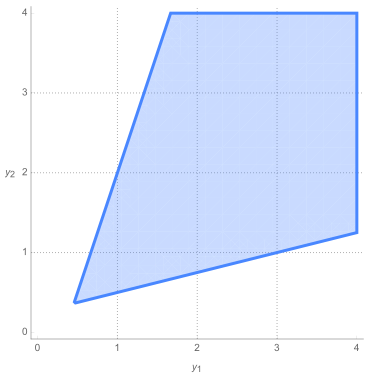
\includegraphics[width=0.5\textwidth]{img/ex2.png}   
    \caption{Přípustná množina řešení k úloze~\ref{eq:P2}.}
    \label{fig:ex2}
\end{figure}

Všimněme si, že v příkladech \ref{eq:P1} a \ref{eq:P2} mají řešení $x^*$ i $y^*$ stejnou cenu. To není náhoda a tento fakt je obsahem silné věty o dualitě lineárního programování, kterou dokázala skupina kolem Alberta W. Tuckera v roce 1948. Začneme slabou větou o dualitě lineárního programování.

\begin{vt}[Slabá o dualitě]
    Nechť $\tilde{x}$ je přípustné řešení \ref{eq:LP-P} a $\tilde{y}$ je přípustné řešení \ref{eq:LP-D}. Potom $c^T \tilde{x} \leq b^T \tilde{y}$.
\end{vt}

Tedy každé přípustné řešení $\tilde{y}$ duální úlohy \ref{eq:LP-D} nám dává horní odhad na maximum účelové funkce primární úlohy \ref{eq:LP-P}. Graficky můžeme slabou větu o dualitě interpretovat jako na obrázku~\ref{fig:weak_duality}. Zatím tedy nevíme, zda vždy existují přípustná (optimální) řešení $x^*$ pro úlohu \ref{eq:LP-P} a $y^*$ pro úlohu \ref{eq:LP-D}, pro která platí $c^T x^* = b^T y^*$. Kladnou odpověď dostaneme z již zmíněné silné věty od dualitě.

\begin{figure}[h!]
    \centering
    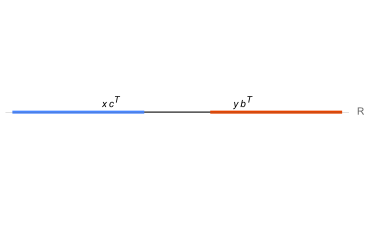
\includegraphics[width=0.5\textwidth]{img/weak_duality.png}   
    \caption{Slabá věta o dualitě.}
    \label{fig:weak_duality}
\end{figure}

\begin{vt}[Silná o dualitě]
    Jestliže úlohy \ref{eq:LP-P} a \ref{eq:LP-D} mají přípustná řešení. Potom
    $$
        \max \left\{ c^T x \mid Ax \leq b, x \geq 0 \right\} = \min \left\{ b^T y \mid A^T y \geq c, y \geq 0 \right\}.
    $$ 
\end{vt}
Se znalostí silné věty o dualitě můžeme obrázek~\ref{fig:weak_duality} upravit na obrázek~\ref{fig:strong_duality}.

\begin{figure}[h!]
    \centering
    \includegraphics[width=0.5\textwidth]{img/strong_duality.png}
    \caption{Ceny přípustných řešení primární a příslušné duální úlohy.}
    \label{fig:strong_duality}
\end{figure}

\section{Komplementární skluzovost}

Pro odvození tzv. podmínky komplementární skluzovosti nejprve převedeme úlohy \ref{eq:LP-P} a \ref{eq:LP-D} do jiných tvarů. V primární úloze povolíme $x \in \mathbb{R}^n$. Tedy primární úloha je ve tvaru:

\begin{equation}\tag{LP-P2}
    \max \left\{ c^T x \mid Ax \leq b \right\}.
    \label{eq:LP-P2}
\end{equation}
A příslušná duální úloha je ve tvaru:

\begin{equation}\tag{LP-D2}
    \min \left\{ b^T y \mid A^T y = c, y \geq 0 \right\}.
    \label{eq:LP-D2}
\end{equation}

Nechť $\tilde{x}$ je připustné řešení a $x^*$ je optimální řešení úlohy \ref{eq:LP-P2}, $\tilde{y}$ je přípustné řešení a $y^*$ je optimální řešení úlohy \ref{eq:LP-D2}. \textbf{Dualitní rozdíl} $\tilde{x}$ a $\tilde{y}$ je číslo $b^T \tilde{y} - c^T \tilde{x} \geq 0$. Ze silné věty o dualitě samozřejmě plyne, že pro optimální řešení $x^*$ a $y^*$ je dualitní rozdíl roven $0$. Vyjdeme z dualitního rozdílu optimálních řešení:
$$
    b^T y^* - c^T x^* = y^{*^T} b - y^{*^T} A x^* = y^{*^T} \left( b - A x^* \right) = 0.
$$
Poslední rovnost přepíšeme maticově:
$$
    \left[ y_1^*, \dots, y_m^* \right] \left(
        \begin{bmatrix}
            b_1    \\
            \vdots \\
            b_m
        \end{bmatrix}
        -
        \begin{bmatrix}
            a_{11} & \dots & a_{1n} \\
            \vdots & \     & \vdots \\
            a_{m1} & \dots & a_{mn}
        \end{bmatrix}
        \begin{bmatrix}
            x_1^*  \\
            \vdots \\
            x_n^*
        \end{bmatrix}
    \right)
    =
    \begin{bmatrix}
    0      \\
    \vdots \\
    0
    \end{bmatrix}.
$$
Dostáváme tedy soustavu rovnic $y_i^* \left( b_i - a_{i\_} x^* \right) = 0$, kde $i = 1, \dots, m$. Tedy buď $y_i^* = 0$ nebo $ b_i - a_{i\_} x^* = 0$. \textbf{Podmínka komplementární skluzovosti} je splněna, jestliže pro přípustná řešení $\tilde{x}, \tilde{y}$ platí buď $\tilde{y}_i = 0$ nebo $b_i - a_{i\_} \tilde{x} = 0$, $i = 1, \dots, m$. Pokud nastane $b_i - a_{i\_} \tilde{x} = 0$, potom říkáme, že \textbf{vazba $a_{i\_} \tilde{x} \leq b_i$ je aktivní}.

\begin{vt}
    Nechť $\tilde{x}$ je přípustné řešení \ref{eq:LP-P2} a $\tilde{y}$ je přípustné řešení \ref{eq:LP-D2}. Potom $\tilde{x}, \tilde{y}$ jsou optimální právě tehdy, když platí podmínka komplementární skluzovosti.
\end{vt}

\section*{TODOs}


\chapter{Semidefinitní programování}

Na semidefinitní programování se můžeme koukat jako na zobecnění lineárního programování, kde proměnné jsou symetrické matice. Jedná se tedy o optimalizaci lineární funkce vzhledem k tzv. lineárním maticovým nerovnostem.

\section{Vsuvka z lineární algebry}

\subsection*{Pozitivně definitní matice}

Pracujeme s reálnými symetrickými maticemi $S = S^T$. Ty mají všechna vlastní čísla reálná a některé z nich mají zajímavou vlastnost, že všechna jejich vlastní čísla jsou kladná. Takovým maticím říkáme, že jsou pozitivně definitní. Alternativní definicí je, že matice $S$ je pozitivně definitní, jestliže $x^TSx > 0$ pro všechny nenulové vektory $x$.

\begin{pr}
$$
    x^T S x = 
    \begin{bmatrix}
        x_1 & x_2
    \end{bmatrix}
    \begin{bmatrix}
        2 & 4 \\
        4 & 9
    \end{bmatrix}
    \begin{bmatrix}
        x_1 \\
        x_2
    \end{bmatrix} =
    2 x_1^2 + 8 x_1 x_2 + 9 x_2^2
$$
Je pro všechny $x$ nenulové $x^TSx > 0$? Ano, protože můžeme výraz přepsat na součet čtverců:
$$
    x^TSx = 2 x_1^2 + 8 x_1 x_2 + 9 x_2^2 = 2 (x_1 + 2 x_2)^2 + x_2^2.
$$
TODO: obrázek kyblíčku
\end{pr}

Ukážeme si několik kritérií, jak otestovat pozitivní definitnost dané matice.

\begin{vt}
    $S = S^T$ je pozitivně definitní, jestliže lze napsat jako $S = A^T A$ pro nějakou matici $A$, která má lineárně nezávislé sloupečky.
\end{vt}
\begin{proof}
    \begin{equation}
    \label{eq:tmp}
        x^TSx = x^TA^TAx = (Ax)^T(Ax) = \lVert Ax \rVert^2 \geq 0
    \end{equation}
    $\lVert Ax \rVert^2 > 0$, jestliže sloupečky matice $A$ jsou lineárně nezávislé
\end{proof}

\begin{pr}
    $$
        S = 
        \begin{bmatrix}
            2 & 3 & 4 \\
            3 & 5 & 7 \\
            4 & 7 & 10
        \end{bmatrix} =
        \begin{bmatrix}
            1 & 1 \\
            1 & 2 \\
            1 & 3
        \end{bmatrix}
        \begin{bmatrix}
            1 & 1 & 1 \\
            1 & 2 & 3
        \end{bmatrix} =
        AA^T
    $$
    $A$ má lineárně závislé sloupečky, tj. $S$ není pozitivně definitní
\end{pr}

Dalším testem je tzv. Sylvesterovo kritérium.

\begin{vt}
    $S = S^T$ je pozitivně definitní, jestliže všechny hlavní minory $S$ jsou kladné.
\end{vt}

\begin{pr}
    $$  S =
        \begin{bmatrix}
            3 & 4 \\
            4 & 6
        \end{bmatrix},
        D_1 = 3,
        D_2 = 3 \cdot 6 - 4 \cdot 4 = 2 
    $$
    hlavní minory $D_1, D_2 > 0$; matice $S$ je pozitivně definitní 
\end{pr}

A poslední, které si uvedeme souvisí s Gaussovou eliminací.

\begin{vt}
    $S = S^T$ je pozitivně definitní, jestliže jsou všechny pivoty při Gaussově eliminaci kladné.
\end{vt}

\begin{pr}
    $$  S =
        \begin{bmatrix}
            3 & 4 \\
            4 & 6
        \end{bmatrix}
        \sim
        \begin{bmatrix}
            3 & 4 \\
            0 & \frac{2}{3}
        \end{bmatrix},
        p_1 = 3, p_2 = \frac{2}{3} 
    $$
    pivoty $p_1, p_2 > 0$; matice $S$ je pozitivně definitní
\end{pr}

\subsection*{Pozitivně semidefinitní matice}

Pro pozitivní semidefinitnost modifikujeme předcházejí definice a tvrzení pro pozitivně definitní matice následovně:
\begin{enumerate}
    \item $S = S^T$ je pozitivně semidefinitní, jestliže všechna její čísla jsou nezáporná.
    \item $S = S^T$ je pozitivně semidefinitní, jestliže $x^TSx \geq 0$ pro všechny nenulové vektory $x$.
    \item $S = S^T$ je pozitivně semidefinitní, jestliže lze napsat jako $S = A^T A$ pro nějakou matici $A$.
    \item $S = S^T$ je pozitivně semidefinitní, jestliže všechny hlavní minory $S$ jsou nezáporné.
    \item $S = S^T$ je pozitivně semidefinitní, jestliže jsou všechny pivoty při eliminaci nezáporné.
\end{enumerate}

\subsection*{Pozitivně semidefinitní kužel}

Množinu všech symetrických matic značíme $S^n$, množinu všech pozitivně semidefinitních matic značíme $S_+^n$ a množinu všech pozitivně definitních matic značíme $S_{++}^n$.

\begin{lm}
    Množina $S_n^+$ je uzavřená
\end{lm}

\begin{proof}
    TODO
\end{proof}

\begin{lm}
    Množina $S_+^n$ tvoří konvexní kužel.
\end{lm}

\begin{proof}
    $\Theta_1, \Theta_2 \geq 0$, $A, B \in S_+^n$
    $$
        x^T \left( \Theta_1 A + \Theta_2 B \right) x = x^T \Theta_1 A x + x^T \Theta_2 B x \geq 0.
    $$
\end{proof}

\begin{lm}
    Kužel $S_+^n$ je pointed.
\end{lm}

\begin{proof}
    TODO
\end{proof}

\begin{lm}
    Kužel $S_+^n$ je samoduální.
\end{lm}

\begin{proof}
    TODO
\end{proof}

\noindent Shrneme předchozí lemmata do následující věty.

\begin{vt}
    Množina $S_+^n$ tvoří konvexní, pointed a uzavřený kužel, který je samoduální.
\end{vt}

Říkáme, že $S_+^n$ je \textbf{pozitivně semidefinitní kužel}.

\subsection*{Spektraedry}

Definujeme tzv. \textbf{L\"{o}wnerovo částečné uspořádání}:
$$
    A \succeq B \iff A - B \in S_+^n,
$$
tj. matice $A - B$ je pozitivně semidefinitní. \textbf{Lineární maticová nerovnost} (LMI) je ve tvaru
$$
    A_0 + \sum_{i=1}^n A_i x_i \succeq 0,
$$
kde $A_i \in S^n$.

Množina $S \subset \mathbb{R}^n$, která je definována pomocí konečně mnoha LMI, se nazývá \textbf{spektraedr}. Tedy:
$$
    S = \left\{ (x_1, \dots, x_m) \in \mathbb{R}^m \mid A_0 + \sum_{i=1}^m A_i x_i \succeq 0 \right\}
$$
pro nějaké symetrické matice $A_0, \dots, A_m \in S^n$.

Můžeme si všimnout analogie s definicí polyedru, který je přípustnou množinu pro lineární program. Podobně spektraedr je přípustnou množinou pro semidefinitní program.

Geometricky je spektraedr definován jako průnik pozitivně semidefinitního kuželu $S_+^n$ a afinního podprostoru $\textbf{span}\left\{ A_1, \dots, A_m \right\}$ posunutého do $A_0$.

Spektraedry jsou uzavřené množiny, neboť LMI je ekvivalentní nekonečně mnoha skalárním nerovnostem ve tvaru $v^T(A_0 + \sum_{i=1}^m A_ix_i)v \geq 0$, jednu pro každou hodnotu $v \in \mathbb{R}^n$.

Vždy můžeme několik LMI \uv{scucnout} do jedné. Stačí zvolit matice $A_i$ blokově diagonální. Odtud snadno vídíme, že polyedr je speciálním případem spektraedru. Polyedr bude mít všechny matice $A_i$ diagonální.

\begin{pr}
    $$
        \left\{ (x, y) \in \mathbb{R}^2 \mid A(x,y) =
        \begin{bmatrix}
            x + 1 & 0      & y \\
            0     & 2      & -x - 1 \\
            y     & -x - 1 & 2
        \end{bmatrix}
        \succeq 0 \right\}
    $$
\end{pr}

\section{Primární úloha}

Semidefinitní program je lineární optimalizační problém přes spektraedr. Primární úlohu ve standardním tvaru můžeme napsat jako:
\begin{equation}\tag{SDP-P}
    \inf \left\{ \langle C, X \rangle \mid \langle A_i, X \rangle = b_i, i=1, \dots, m; X \succeq 0 \right\},
    \label{eq:SDP-P}
\end{equation}
kde $C, A_i \in S^n$, $\langle X, Y \rangle = \textbf{Tr}(X^T Y) = \sum_{ij} X_{ij}Y_{ij}$ a $X \in S^n$ je proměnná, nad kterou provádíme minimalizaci.

\begin{pr}
    \begin{equation}\tag{P3}
        \inf \left\{
            \left\langle
            \begin{bmatrix}
                2 & 1 \\
                1 & 0
            \end{bmatrix},
            \begin{bmatrix}
                x_{11} & x_{12} \\
                x_{12} & x_{22}
            \end{bmatrix}
            \right\rangle \middle|
            \left\langle
            \begin{bmatrix}
                1 & 0 \\
                0 & 1
            \end{bmatrix},
            \begin{bmatrix}
                x_{11} & x_{12} \\
                x_{12} & x_{22}
            \end{bmatrix}
            \right\rangle = 1,
            \begin{bmatrix}
                x_{11} & x_{12} \\
                x_{12} & x_{22}
            \end{bmatrix} \succeq 0
        \right\}
        \label{eq:P3}
    \end{equation}
    Po úpravě:
    $$
        \inf \left\{
            2 x_{11} + 2 x_{12} \middle| x_{11} + x_{22} = 1, 
            \begin{bmatrix}
                x_{11} & x_{12} \\
                x_{12} & x_{22}
            \end{bmatrix} \succeq 0
        \right\}.
    $$
    Jak vypadá přípustná množina? Použijeme Sylvesterovo kritérium, tj.
    $$
        x_{11} \geq 0, x_{11} x_{22} - x_{12}^2 \geq 0.
    $$
    Z LMI vyjádříme $x_{22}$, tj.
    $$
        x_{22} = 1 - x_{11}
    $$
    Dosadíme do přechozího a dostaneme
    $$
        x_{11} \geq 0, x_{11} \left(1 - x_{11}\right) - x_{12}^2 \geq 0
    $$
    Po úpravě
    $$
        x_{11} \geq 0, \left(x_{11} - \frac{1}{2}\right)^2 + x_{12}^2 \leq \frac{1}{4}
    $$
    Vidíme tedy, že přípustná množina (zobrazena na obrázku~\ref{fig:ex3}) je kruh s poloměrem $\frac{1}{2}$ a se středem v bodě $(x_{11}, x_{12}) = (\frac{1}{2}, 0)$. Řešením úlohy je matice
    $$
        X^* \approx
        \begin{bmatrix}
            0.1464  & -0.3536 \\
            -0.3536 &  0.8536
        \end{bmatrix}
    $$
    s cenou $\approx -0.4142$. Implementace v softwaru MOSEK: \url{https://github.com/c0n73x7/D1PL0MK4/blob/master/mosek/ex3.py}.
\end{pr}

\begin{figure}[h!]
    \centering
    \includegraphics[width=0.5\textwidth]{img/ex3.png}   
    \caption{Přípustná množina řešení k úloze~\ref{eq:P3}.}
    \label{fig:ex3}
\end{figure}

\section{Dualita}

\subsubsection*{Duální úloha}

Podobně jako u lineárního programování použijeme Lagrangeovu dualitu k odvození duální úlohy k úloze~\ref{eq:SDP-P}. Lagrangeova funkce je ve tvaru:
$$
    L(X, \lambda, Z) = \langle C, X \rangle - \sum_{i=1}^m \lambda_i \left( \langle A_i, X \rangle - b_i \right) - \langle Z, X \rangle.
$$

\noindent K ní duální funkce:
$$
    d(\lambda, Z) = \inf_{X \in S^n} L(X, \lambda, Z) = 
    \begin{cases}
        \lambda^T b & \dots\ C - \sum_{i=1}^m \lambda_i A_i - Z = 0, \\
        -\infty     & \dots\ \text{jinak.}
    \end{cases}
$$

\noindent Duální funkci použijeme v duální úloze:
\begin{equation}\tag{SDP-D}
    \sup\left\{ \lambda^Tb \mid C - \sum_{i=1}^m \lambda_i A_i \succeq 0 \right\},
    \label{eq:SDP-D}
\end{equation}
kde $\lambda = (\lambda_1, \dots, \lambda_m)$ je duální proměnná.

\noindent Dostali jsme duální úlohu~\ref{eq:SDP-D} k úloze~\ref{eq:SDP-P}.

\subsubsection*{Slabá dualita semidefinitního programování}

Vztah mezi primární a duální úlohou je podobně jako u lineárního programování v tom, že řešení jedné úlohy lze použít jako odhad na úlohu druhou. Nechť $X$ je libovolné přípustné řešení primární úlohy a $y$ je libovolné přípustné řešení duální úlohy. Potom
$$
    \langle C, X \rangle - b^T y =
    \langle C, X \rangle - \sum_{i=1}^m y_i \langle A_i, X \rangle =
    \left\langle C - \sum_{i=1}^m A_i y_i, X \right\rangle \geq 0
$$

\subsubsection*{Silná dualita semidefinitního programování}



\section*{WIP}

Stopa matice $A \in R^{n \times n}$ je $\textbf{Tr}(A) = \sum_{i=1}^n A_{ii}$.

\begin{vt}
$S, T$ jsou pozitivně definitní $\implies$ $S + T$ je pozitivně definitní
\end{vt}

\begin{proof}
$x^T (S+T) x = x^T S x + x^T T x > 0$
\end{proof}


\noindent Úlohy s racionálními daty nemusí mít racionální optimální řešení.
\noindent příklad

\noindent Jen 3 kužely s vlastnostmi jako PSD cone. Zmrzlina, a ještě jeden.
\noindent Vnitřek $S_+^n$ je $S_{++}^n$.


%spektraedr, formulace, dualita, semidefinitní kužel, duální kužel, ...
%vektorové programování a jeho ekvivalence, formulace úloh

\chapter{Kombinatorická optimalizace}

\section{Celočíselné lineární programování}

složitost úlohy, relaxace, výčet algoritmů, aproximace, ...

\section{Celočíselné semidefinitní programování}

složitost úlohy, relaxace, výčet algoritmů, aproximace, ...

\clearpage


% ------------------------- ČÁST: KOMBINATORICKÉ ÚLOHY ----------------------- %
\part{Kombinatorické úlohy}

\input{kapitoly/06_shannonova_kapacita}

\chapter{Problém maximálníhu řezu}

\section{Kvadratické programování}

kvadratický program, striktní kvadratický program

\section{Relaxace a vektorové programování}

ekvivalence se semidefinitním programováním

\section*{TODO}

formulace úlohy, approximační algoritmy, porovnání semidefinitních programů, ...
komplexní semidefinitní programování, ...

\input{kapitoly/08_obchodni_cestujici}

\clearpage


% ---------------------------------- Závěr ----------------------------------- %
\chapter*{Závěr}
\addcontentsline{toc}{chapter}{Závěr}

V prvních čtyřech kapitolách je shrnuta teorie, která se dále využívá při popisu úloh kombinatorické optimalizace.

V kapitole o Shannonově kapacitě se věnujeme Lovászově $\vartheta$ funkci a jejímu využití. Byly naimplementovány a následně porovnány dva modely s přesnou hodnotou pro liché kružnice. Jednodušší model, který dává rovnou hodnotu $\vartheta$ funkce byl přesnější. U druhého modelu, ze kterého dostaneme hodnotu $1/\sqrt{\vartheta}$, byly patrné chyby už pro malé grafy. Problémem je, že úloha není ve standardním tvaru a frameworky typu Mosek jsou optimalizovány hlavně na práci s úlohami ve standardním tvaru. Dále byl puštěn výpočet pro vylepšení dolního odhadu Shannonovy kapacity kružnice $C_7$, ale nezávislá množina, která by odhad vylepšila se nenašla.

Pro úlohu MAX $k$-CUT byly pro účely testování implementovány čtyři algoritmy a pro úlohu kapacitního MAX $k$-CUTu další dva. U experimentu pro úlohu MAX $3$-CUT vyšel nejhůře algoritmus~\ref{alg:gw-max-3-cut}, který má nejlepší aproximační poměr, což je to dáno složitostí modelu založeného na komplexním semidefinitním programování, který je třikrát větší než model použitý v ostatních algoritmech a navíc obsahuje hodně omezení (vznikaly zaokrouhlovací chyby). Pro MAX $4$-CUT a MAX $5$-CUT vyšel nejlépe algoritmus~\ref{alg:n-max-k-cut-2}, který je jen navrhnut v závěru článku \cite{newman} a není pro něj znám aproximační poměr. U~kapacitní verze byly porovnány dva přístupy: algoritmus založený na lokálním prohledávání a náš algoritmus využívající semidefinitní programování. Oba algoritmy dávaly srovnatelné výsledky, ale rozdíl byl hlavně v době běhu, kde jasně vyhrává algoritmus využívající lokální prohledávání. Algoritmus založený na semidefinitní programování dával lepší výsledky, když součet kapacit jednotlivých množin byl větší než počet vrcholů grafu. 

Dále by mohla být věnována pozornost analýze algoritmu~\ref{alg:n-max-k-cut-2}, o kterém není známé nic.

Celá práce i s implementacemi je dostupná na \url{https://github.com/c0n73x7/D1PL0MK4}.

\clearpage


% ---------------------------- Použitá literatura ---------------------------- %
\bibliography{citace}
\bibliographystyle{plain}

\end{document}
